\documentclass[12pt]{article}

% --------------------
% PAQUETES
% --------------------
\usepackage[spanish]{babel}
\usepackage[utf8]{inputenc}
\usepackage[T1]{fontenc}
\usepackage{graphicx}
\usepackage{float}
\usepackage{caption}
\usepackage{subcaption}
\usepackage{geometry}
\usepackage{setspace}

% --------------------
% CONFIGURACIÓN DE PÁGINA
% --------------------
\geometry{
	a4paper,
	left=2.5cm,
	right=2.5cm,
	top=2.5cm,
	bottom=2.5cm
}

\onehalfspacing

% --------------------
% DOCUMENTO
% --------------------
\begin{document}
	
	% --------------------
	% TÍTULO PRINCIPAL
	% --------------------
	\begin{center}
		{\LARGE \textbf{Título Principal del Documento}}\\[1em]
	\end{center}
	
	% --------------------
	% DESCRIPCIÓN GENERAL
	% --------------------
	\noindent
	Esta sección presenta una descripción general del contenido del documento. 
	Aquí se explica brevemente el objetivo del trabajo, el contexto en el que se 
	desarrolla y la importancia de las imágenes que se presentan a continuación.
	
	\vspace{1cm}
	
	% =====================================================
	% SECCIÓN DE IMÁGENES (2 IMÁGENES POR HOJA)
	% =====================================================
	
	% ---------- HOJA 1 ----------
	\begin{figure}[H]
		\centering
		\begin{minipage}{0.48\textwidth}
			\centering
			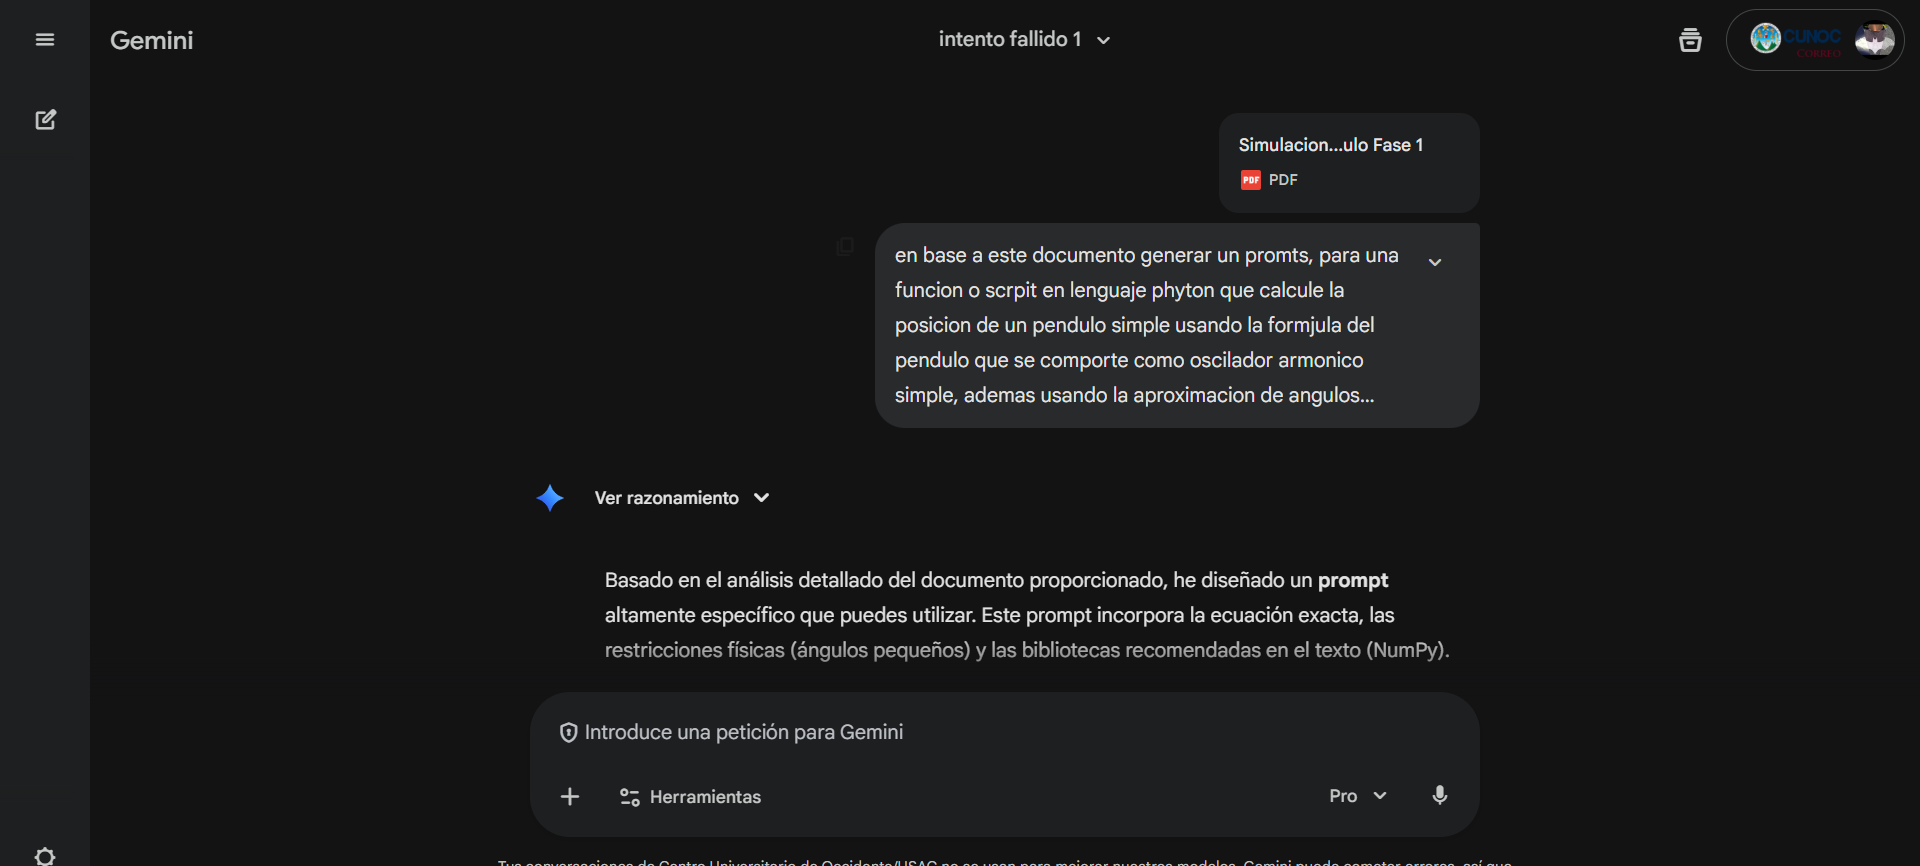
\includegraphics[width=\linewidth,height=0.45\textheight]{imagen1}
			\caption{Descripción de la imagen 1.}
		\end{minipage}
		\hfill
		\begin{minipage}{0.48\textwidth}
			\centering
			
			\caption{Descripción de la imagen 2.}
		\end{minipage}
	\end{figure}
	
	\clearpage
	
	% ---------- HOJA 2 ----------
	\begin{figure}[H]
		\centering
		\begin{minipage}{0.48\textwidth}
			\centering
		
			\caption{Descripción de la imagen 3.}
		\end{minipage}
		\hfill
		\begin{minipage}{0.48\textwidth}
			\centering
		
			\caption{Descripción de la imagen 4.}
		\end{minipage}
	\end{figure}
	
	\clearpage
	
	% ---------- HOJA 3 ----------
	\begin{figure}[H]
		\centering
		\begin{minipage}{0.48\textwidth}
			\centering
			
			\caption{Descripción de la imagen 5.}
		\end{minipage}
		\hfill
		\begin{minipage}{0.48\textwidth}
			\centering
		
			\caption{Descripción de la imagen 6.}
		\end{minipage}
	\end{figure}
	
	\clearpage
	
	% ---------- HOJA 4 ----------
	\begin{figure}[H]
		\centering
		\begin{minipage}{0.48\textwidth}
			\centering
			
			\caption{Descripción de la imagen 7.}
		\end{minipage}
		\hfill
		\begin{minipage}{0.48\textwidth}
			\centering
		
			\caption{Descripción de la imagen 8.}
		\end{minipage}
	\end{figure}
	
	\clearpage
	
	% ---------- HOJA 5 ----------
	\begin{figure}[H]
		\centering
		\begin{minipage}{0.48\textwidth}
			\centering
		
			\caption{Descripción de la imagen 9.}
		\end{minipage}
		\hfill
		\begin{minipage}{0.48\textwidth}
			\centering
		
			\caption{Descripción de la imagen 10.}
		\end{minipage}
	\end{figure}
	
	\clearpage
	
	% ---------- HOJA 6 ----------
	\begin{figure}[H]
		\centering
		\begin{minipage}{0.48\textwidth}
			\centering
		
			\caption{Descripción de la imagen 11.}
		\end{minipage}
		\hfill
		\begin{minipage}{0.48\textwidth}
			\centering
			
			\caption{Descripción de la imagen 12.}
		\end{minipage}
	\end{figure}
	
	\clearpage
	
	% ---------- HOJA 7 ----------
	\begin{figure}[H]
		\centering
		\begin{minipage}{0.48\textwidth}
			\centering
		
			\caption{Descripción de la imagen 13.}
		\end{minipage}
		\hfill
		\begin{minipage}{0.48\textwidth}
			\centering
			
			\caption{Descripción de la imagen 14.}
		\end{minipage}
	\end{figure}
	
	\clearpage
	
	% ---------- IMAGEN 15 (CENTRADA) ----------
	\begin{figure}[H]
		\centering
		
		\caption{Descripción de la imagen 15.}
	\end{figure}
	
	\clearpage
	
	% =====================================================
	% SECCIÓN FINAL
	% =====================================================
	\section{Conclusión o Comentarios Finales}
	
	En esta sección se presenta un breve texto descriptivo que resume el contenido 
	mostrado a través de las imágenes. Se pueden destacar observaciones importantes, 
	conclusiones generales o recomendaciones derivadas del análisis visual presentado 
	en el documento.
	
\end{document}
